\documentclass[10pt]{article}
\usepackage[UTF8]{ctex}

\usepackage[utf8]{inputenc} % allow utf-8 input
\usepackage{amsthm}
\usepackage{amsmath,amscd}
\usepackage{amssymb,array}
\usepackage{amsfonts,latexsym}
\usepackage{graphicx,subfig,wrapfig}
\usepackage{times}
\usepackage{psfrag,epsfig}
\usepackage{verbatim}
\usepackage{tabularx}
\usepackage[pagebackref=true,breaklinks=true,letterpaper=true,colorlinks,bookmarks=false]{hyperref}
\usepackage{cite}
\usepackage{algorithm}
\usepackage{multirow}
\usepackage{caption}
\captionsetup[figure]{labelformat=default,labelsep=period,name=Figure}

\usepackage{algorithmic}
%\usepackage[amsmath,thmmarks]{ntheorem}
\usepackage{listings}
\usepackage{color}
\usepackage{bm}

% support llbracket and rrbracket  []
\usepackage{stmaryrd}


\newtheorem{thm}{Theorem}
\newtheorem{mydef}{Definition}

\DeclareMathOperator*{\rank}{rank}
\DeclareMathOperator*{\trace}{trace}
\DeclareMathOperator*{\acos}{acos}
\DeclareMathOperator*{\argmax}{argmax}


\renewcommand{\algorithmicrequire}{ \textbf{Input:}}
\renewcommand{\algorithmicensure}{ \textbf{Output:}}
\renewcommand{\mathbf}{\boldsymbol}
\newcommand{\mb}{\mathbf}
\newcommand{\matlab}[1]{\texttt{#1}}
\newcommand{\setname}[1]{\textsl{#1}}  
\newcommand{\Ce}{\mathbb{C}}
\newcommand{\Ee}{\mathbb{E}}
\newcommand{\Ne}{\mathbb{N}}
\newcommand{\Se}{\mathbb{S}}
\newcommand{\norm}[2]{\left\| #1 \right\|_{#2}}

\newenvironment{mfunction}[1]{
	\noindent
	\tabularx{\linewidth}{>{\ttfamily}rX}
	\hline
	\multicolumn{2}{l}{\textbf{Function \matlab{#1}}}\\
	\hline
}{\\\endtabularx}

\newcommand{\parameters}{\multicolumn{2}{l}{\textbf{Parameters}}\\}

\newcommand{\fdescription}[1]{\multicolumn{2}{p{0.96\linewidth}}{

		\textbf{Description}

		#1}\\\hline}

\newcommand{\retvalues}{\multicolumn{2}{l}{\textbf{Returned values}}\\}
\def\0{\boldsymbol{0}}
\def\b{\boldsymbol{b}}
\def\bmu{\boldsymbol{\mu}}
\def\e{\boldsymbol{e}}
\def\u{\boldsymbol{u}}
\def\x{\boldsymbol{x}}
\def\v{\boldsymbol{v}}
\def\w{\boldsymbol{w}}
\def\N{\boldsymbol{N}}
\def\X{\boldsymbol{X}}
\def\Y{\boldsymbol{Y}}
\def\A{\boldsymbol{A}}
\def\B{\boldsymbol{B}}
\def\y{\boldsymbol{y}}
\def\cX{\mathcal{X}}
\def\transpose{\top} % Vector and Matrix Transpose

%\long\def\answer#1{{\bf ANSWER:} #1}
\long\def\answer#1{}
\newcommand{\myhat}{\widehat}
\long\def\comment#1{}
\newcommand{\eg}{{e.g.,~}}
\newcommand{\ea}{{et al.~}}
\newcommand{\ie}{{i.e.,~}}

\newcommand{\db}{{\boldsymbol{d}}}
\renewcommand{\Re}{{\mathbb{R}}}
\newcommand{\Pe}{{\mathbb{P}}}

\hyphenation{MATLAB}

\usepackage[margin=1in]{geometry}

\newcounter{ProblemCounter}
\newcounter{oldvalue}
\newcommand{\problem}[2][-1]{
	\setcounter{oldvalue}{\value{secnumdepth}}
	\setcounter{secnumdepth}{0}
	\ifnum#1>0
		\setcounter{ProblemCounter}{#1}
	\else
		\stepcounter{ProblemCounter}
	\fi
	\section{Problem \arabic{ProblemCounter}: #2}
	\setcounter{secnumdepth}{\value{oldvalue}}
}
\newcommand{\subproblem}[1]{
	\setcounter{oldvalue}{\value{section}}
	\setcounter{section}{\value{ProblemCounter}}
	\subsection{#1}
	\setcounter{section}{\value{oldvalue}}
}



\begin{document}

\title{	Digital Image Processing, 2024 Spring\\Homework 2}
\date{Due 23:59 (CST), May. 3, 2024 }

\author{
    Name: \textbf{Zhou Shouchen} \\
	Student ID: 2021533042
}

\maketitle

\newpage
%===============================
\problem{Image Sharping}
(a) Let $\mathbf{a}=\begin{bmatrix}-1 & 0 & 1\end{bmatrix}^T$, and $\mathbf{b}=\begin{bmatrix}1 & 2 & 1\end{bmatrix}^T$.

Sobel operator among $x$ direction:
$S_x=\begin{bmatrix}
    -1 & -2 & -1 \\
    0 & 0 & 0 \\
    1 & 2 & 1
\end{bmatrix}=\begin{bmatrix}-1 \\ 0 \\ 1\end{bmatrix}\begin{bmatrix}1 & 2 & 1\end{bmatrix}= \mathbf{a}\mathbf{b}^T$

Sobel operator among $y$ direction:
$S_y=\begin{bmatrix}
    -1 & 0 & 1 \\
    -2 & 0 & 2 \\
    -1 & 0 & 1
\end{bmatrix}=\begin{bmatrix}1 \\ 2 \\ 1\end{bmatrix}\begin{bmatrix}-1 & 0 & 1\end{bmatrix}= \mathbf{b}\mathbf{a}^T$\\
So both the Sobel operators can be represented as the outer product of two vectors, i.e. its separable.\\
From what we have learned, if a separable filter can be represented as $\mathbf{w}= \mathbf{w}_1\mathbf{w}_2^T$, then the convolution of the filter with an image can be computed as $\mathbf{I}*\mathbf{w}=(\mathbf{I}*\mathbf{w}_1)*\mathbf{w}_2^T$, where `$*$' represents convolution.\\
So we can implement the separated kernels sequencially to the origin image to get the results.\\
The $S\_x\_a$ represents the convolution of origin image and $\mathbf{a}$, $S\_x\_ab$ represents convolution of $S\_x\_a$ and $\mathbf{b}^T$, which also means that the convolution of origin image and the $S_x$ operator.\\
And $S\_y\_b$ represents the convolution of origin image and $\mathbf{b}$, $S\_y\_ba$ represents convolution of $S\_y\_b$ and $\mathbf{a}^T$, which also means that the convolution of origin image and the $S_y$ operator.\\
Specifically, for the convenience of checking, the negative values are turned to $0$, and then the image pixel values are normalized to $[0, 255]$ after filtering.\\
And the results are shown in Figure \ref{fig:p1a}.\\

\begin{figure}[htbp]
    \centering
	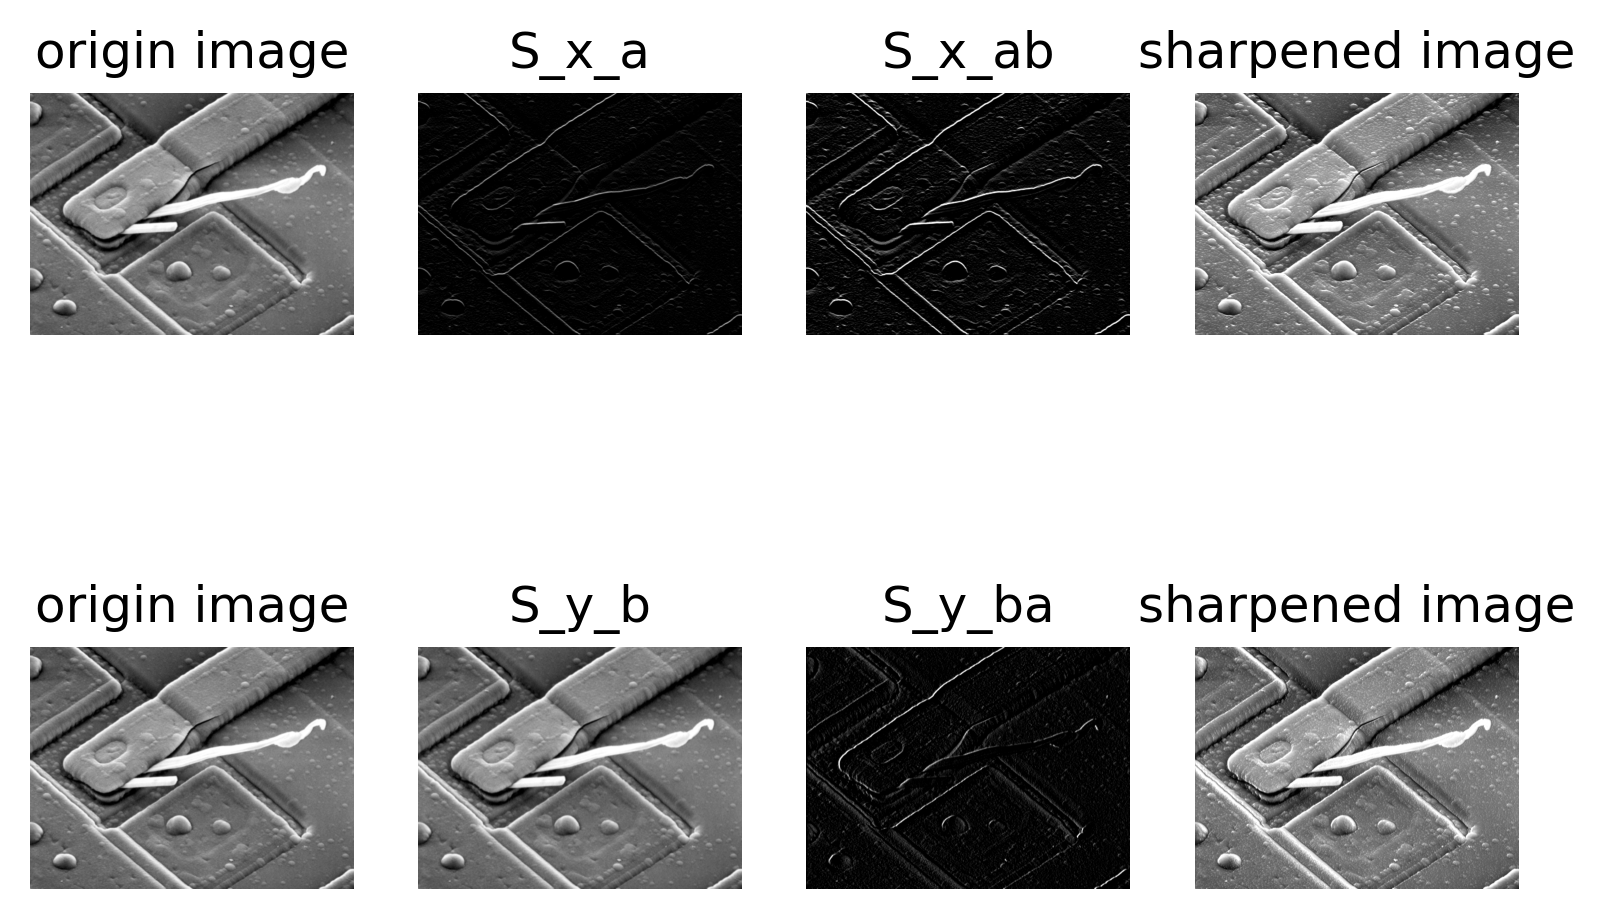
\includegraphics[width=\textwidth]{../images/p1/p1a.png}
    \caption{Processed images by Sobel operators among $x$ and $y$ directions.}
    \label{fig:p1a}
\end{figure}
We also tried to use the gradient of Sobel kernels to sharpen the image.\\
i.e.
$$G = \sqrt{(S\_x\_ab)^2 + (S\_y\_ba)^2}$$
The gradient of Sobel kernels and its sharpened image are shown in Figure \ref{fig:p1a_gradient}.\\
\begin{figure}[htbp]
    \centering
	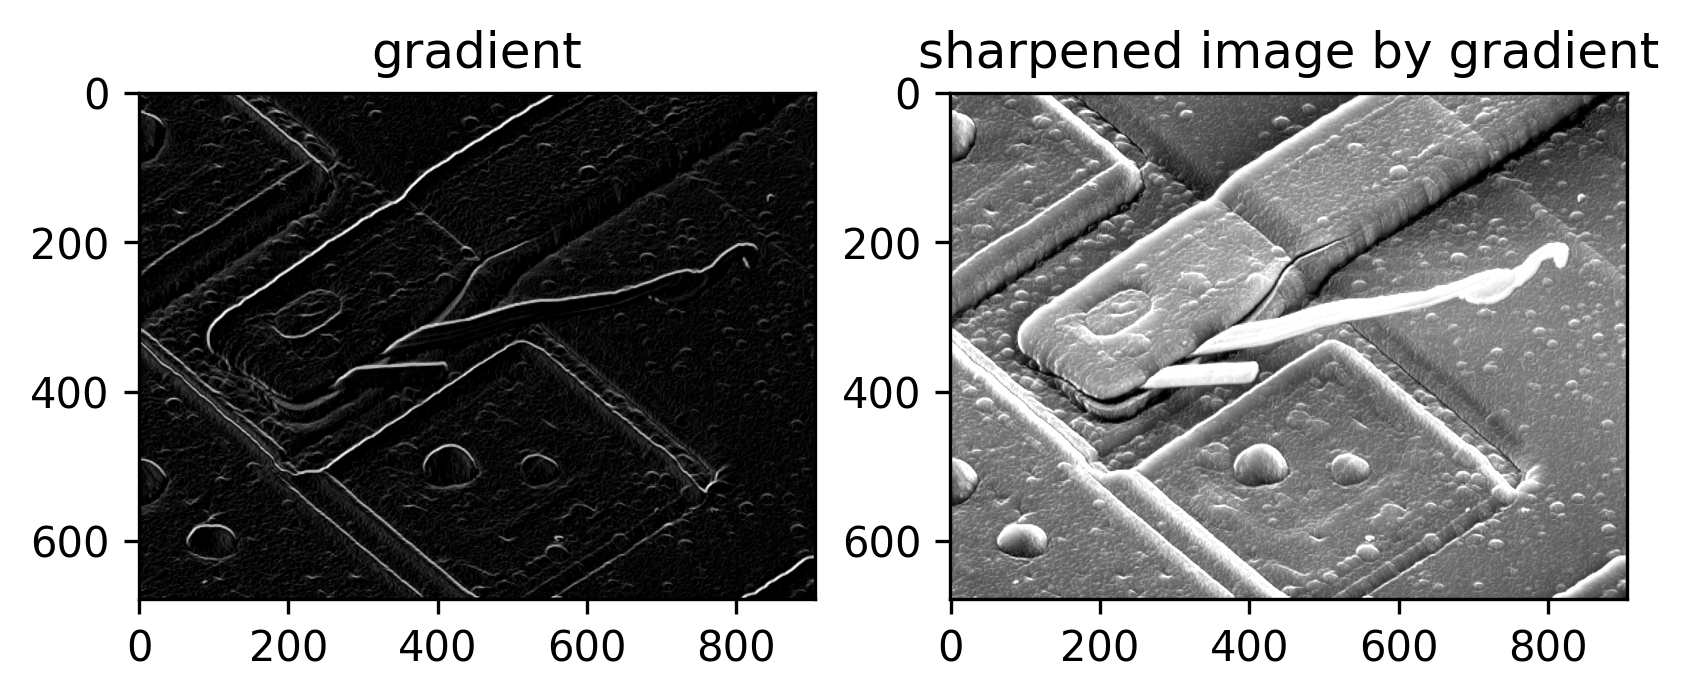
\includegraphics[width=\textwidth]{../images/p1/p1a_gradient.png}
    \caption{Sharpened by the gradient of Sobel kernels.}
    \label{fig:p1a_gradient}
\end{figure}


(b) Gaussian Highpass Filter:\\
The Gaussian Highpass Filter is:
$$H(u,v)=1-\exp\left(-\dfrac{D(u,v)^2}{2D_0^2}\right)$$
Where
$$D(u,v)=\left[\left(u-\dfrac{P}{2}\right)^2+\left(v-\dfrac{Q}{2}\right)^2\right]^\frac{1}{2}$$
In order to do FFT, we need to pad the image to the size of $2^m*2^n$, where $m$ and $n$ are integers.\\
So the images size varies: $678*906\Rightarrow 1024*1024$.
And aftering filtering, the image is cropped to the original size.

The Gaussian high pass filter is shown in Figure \ref{fig:p1b_Gaussian}.\\

\begin{figure}[htbp]
    \centering
	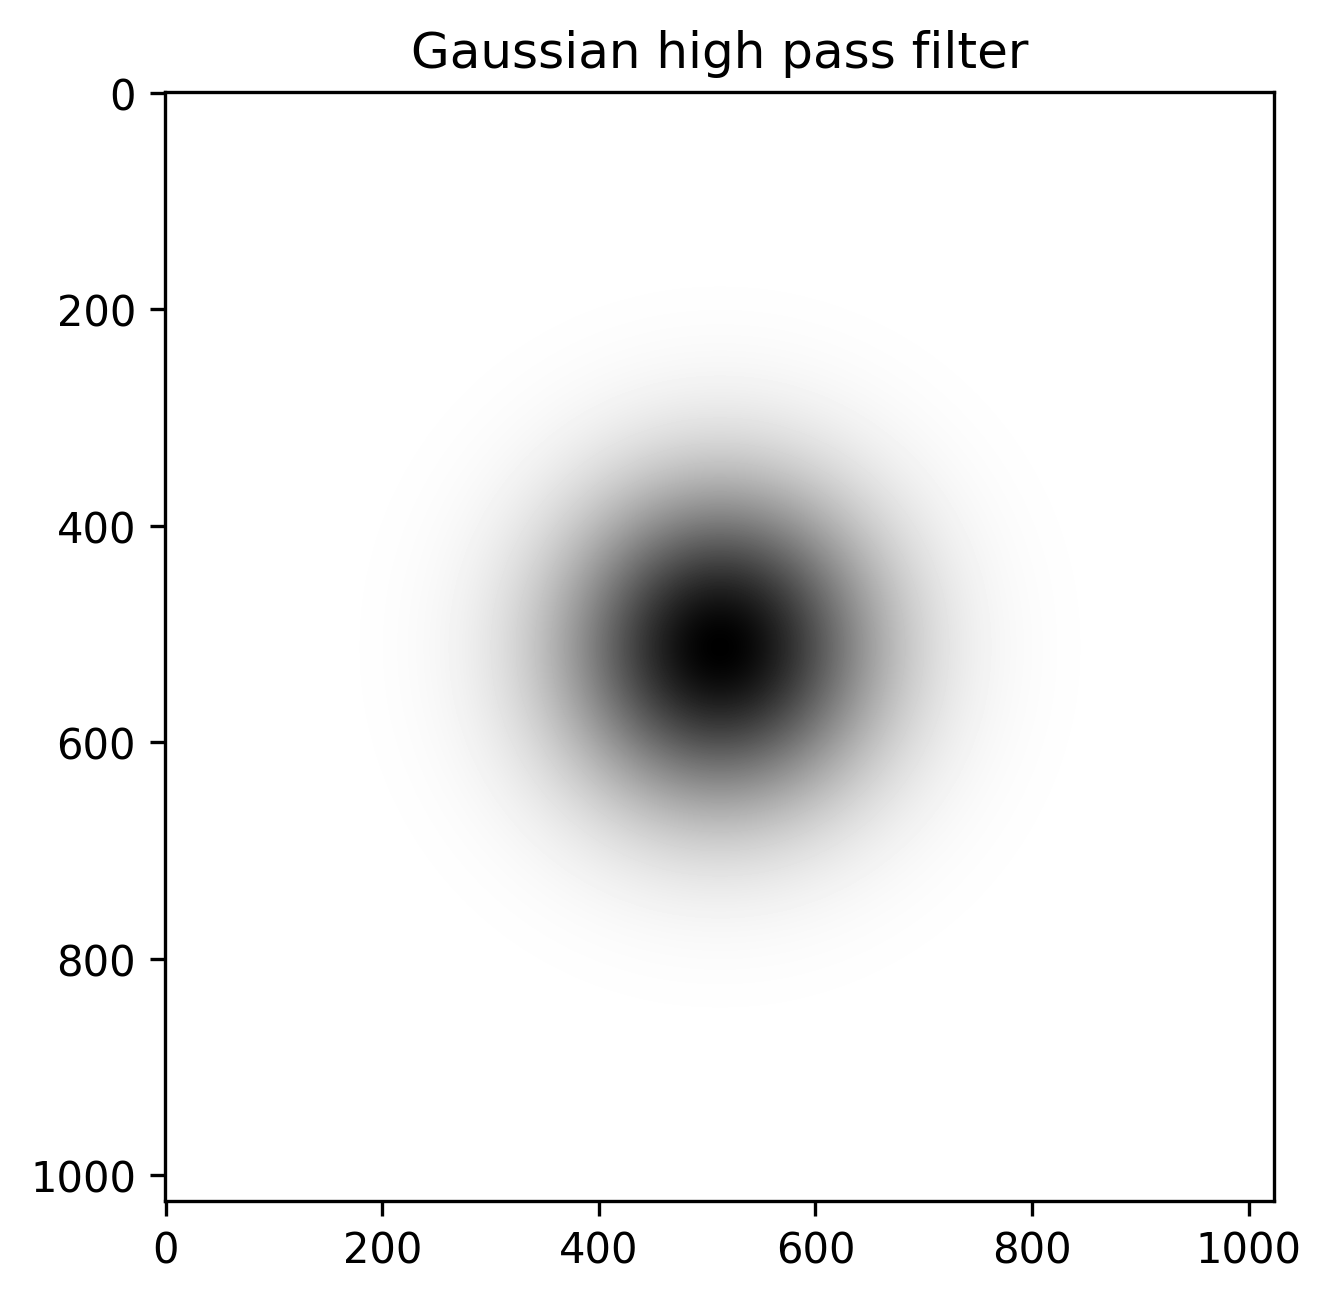
\includegraphics[width=0.4\textwidth]{../images/p1/p1b_Gaussian.png}
	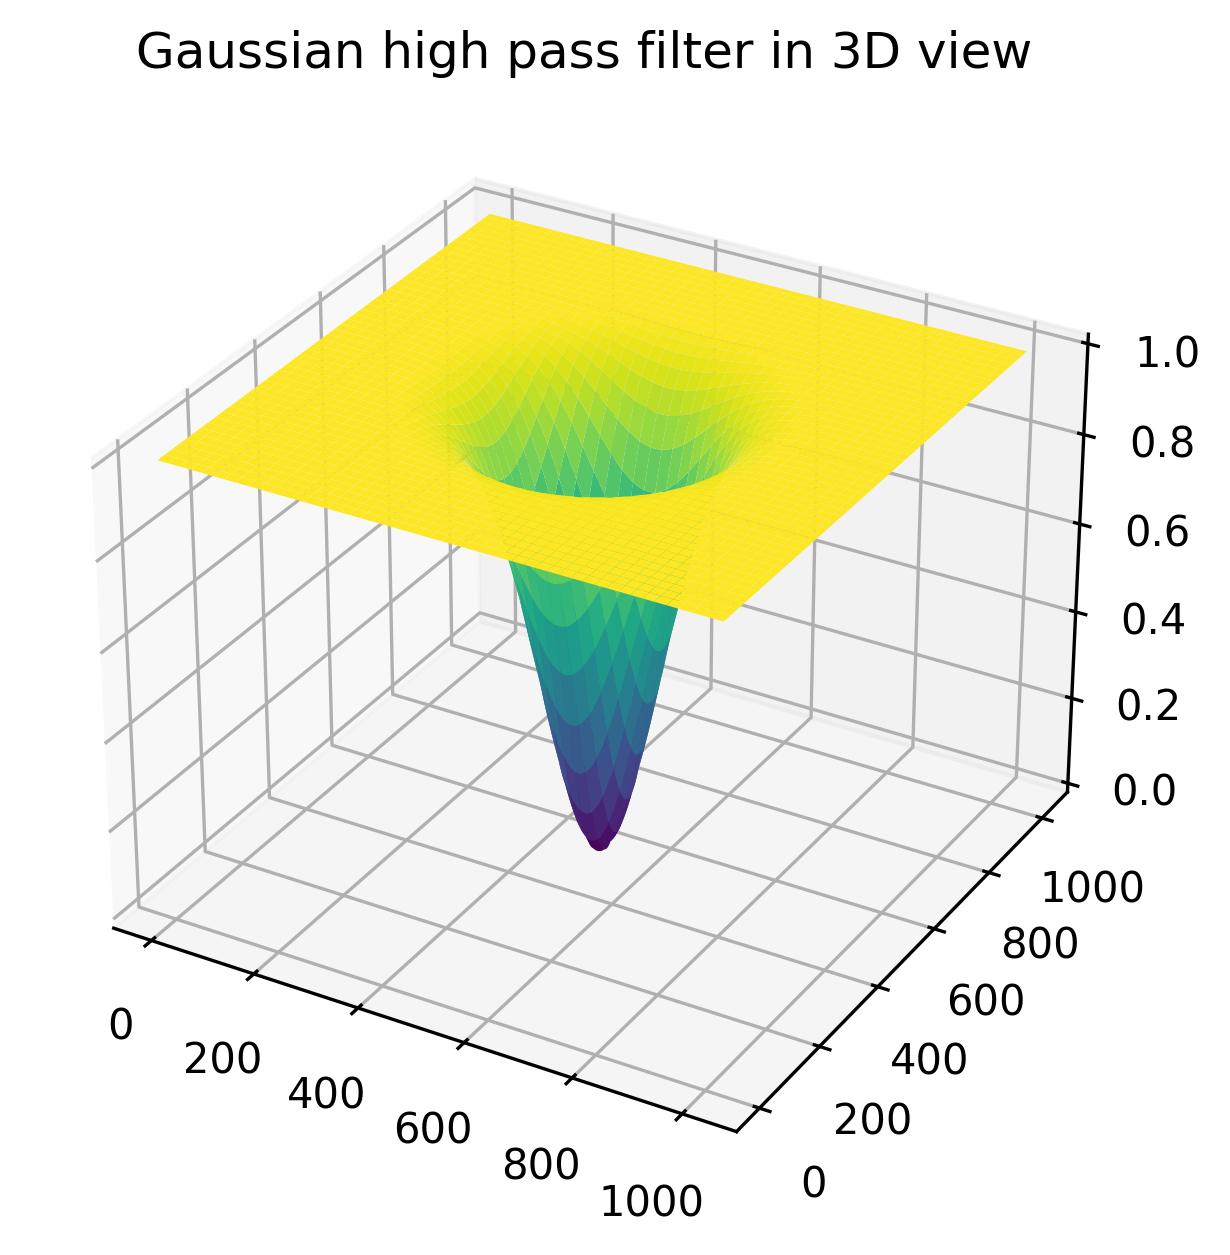
\includegraphics[width=0.4\textwidth]{../images/p1/p1b_Gaussian_3D.png}
    \caption{Gaussian high pass filter}
    \label{fig:p1b_Gaussian}
\end{figure}


To have a better effect of visualization on the frequency domain, the image is shown by applying the log transformation on the magnitude of the Fourier transform of the image.\\
i.e. $I_{\text{log}}=20\log(1+|I|)$, where $I$ is the spectrum generated by Fourier transform of the image.\\
The spectrum of the origin image and its filtered spectrum by the Gaussian highpass filter is shown in Figure \ref{fig:p1b_spectrum}.\\
The results of filtering the image with the Gaussian high pass filter and its sharpened image is shown in Figure \ref{fig:p1b_result}.\\
The filtered image is generated by using the inverse Fourier transform to the frequency domain results in the real domain.\\

\begin{figure}[htbp]
    \centering
	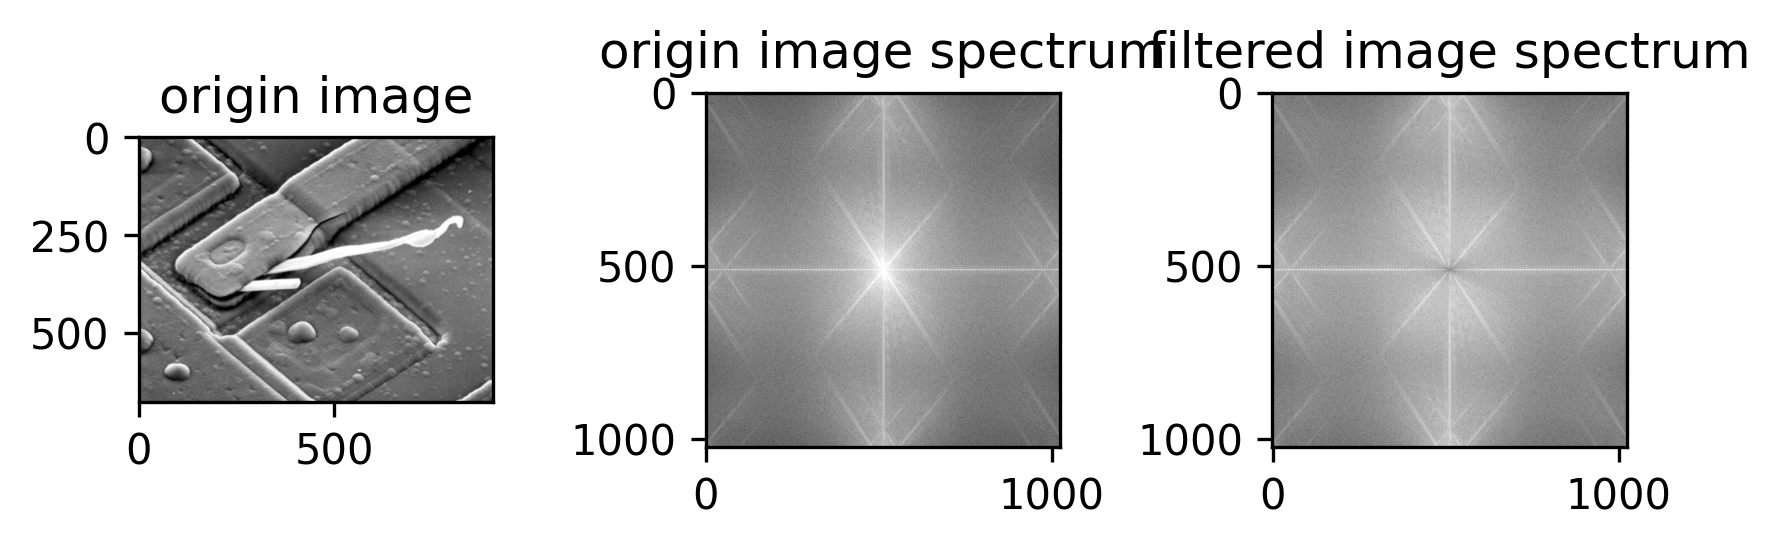
\includegraphics[width=\textwidth]{../images/p1/p1b_spectrum.png}
    \caption{Spectrum of Gaussian Highpass Filtered iamge.}
    \label{fig:p1b_spectrum}
\end{figure}

\begin{figure}[htbp]
    \centering
	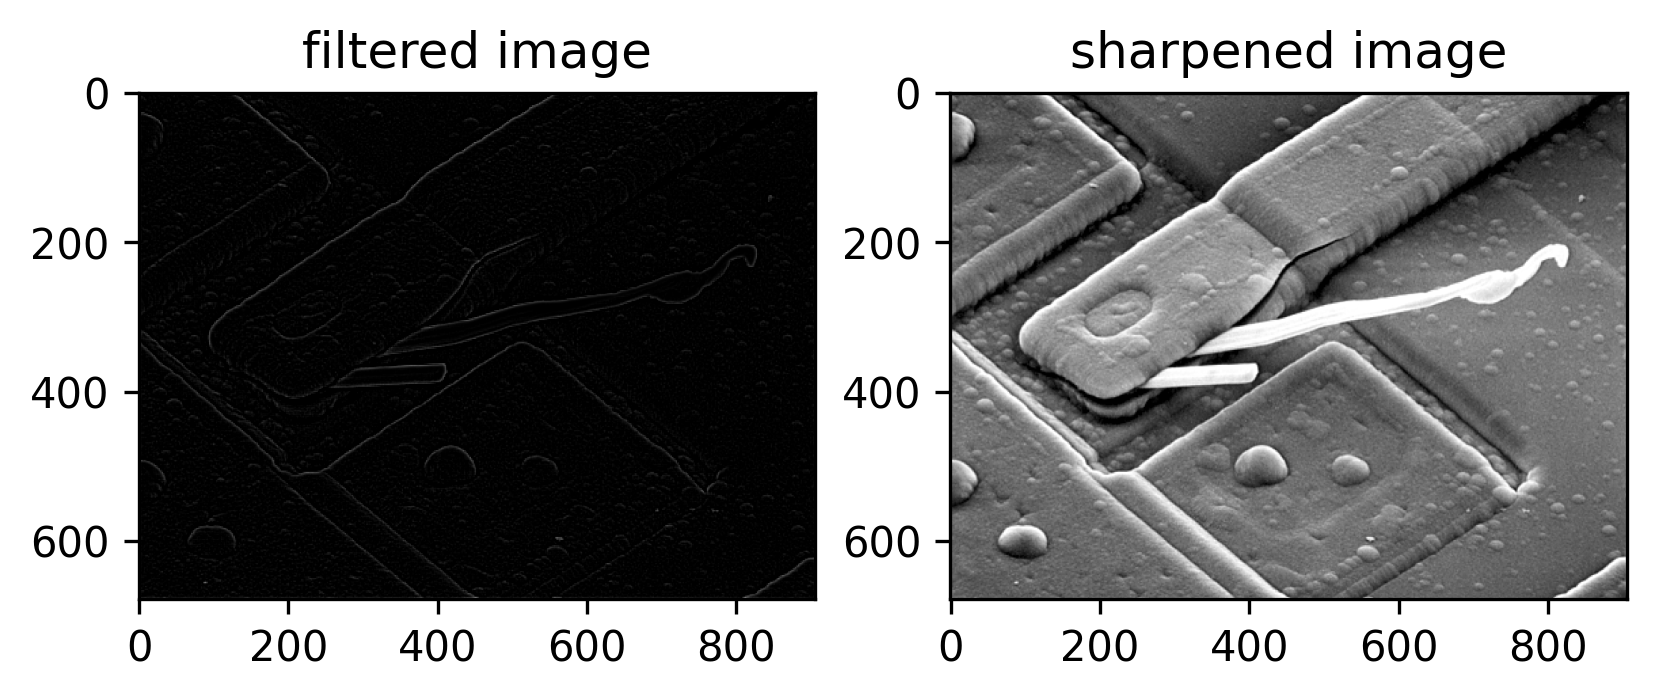
\includegraphics[width=0.9\textwidth]{../images/p1/p1b_result.png}
    \caption{Results of filtering the image with the Gaussian high pass filter.}
    \label{fig:p1b_result}
\end{figure}

\newpage
\problem{}
For the details of this problem: the image is padded with the edge values during the convolution, since during the convolution process, it may need to access the pixels outside the image.

(a) The Laplacian kernel is that:
$$
\nabla^2 f = \begin{bmatrix}
    0 & 1 & 0 \\
    1 & -4 & 1 \\
    0 & 1 & 0
\end{bmatrix}
=
\begin{bmatrix}
    0 & 1 & 0 \\
    0 & -2 & 0 \\
    0 & 1 & 0
\end{bmatrix}
+
\begin{bmatrix}
    0 & 0 & 0 \\
    1 & -2 & 1 \\
    0 & 0 & 0
\end{bmatrix}
$$
We can seperate the Laplcian kernel along the $x$-direction and $y$-direction, and we can simplify them into 1-D:

$$\begin{bmatrix}1\\-2\\1\end{bmatrix} \text{\ \ and \ \ } \begin{bmatrix}1 & -2 & 1\end{bmatrix}$$

The processed image corresponding to the kernel above all shown in Figure \ref{fig:p2a}.\\

\begin{figure}[htbp]
    \centering
	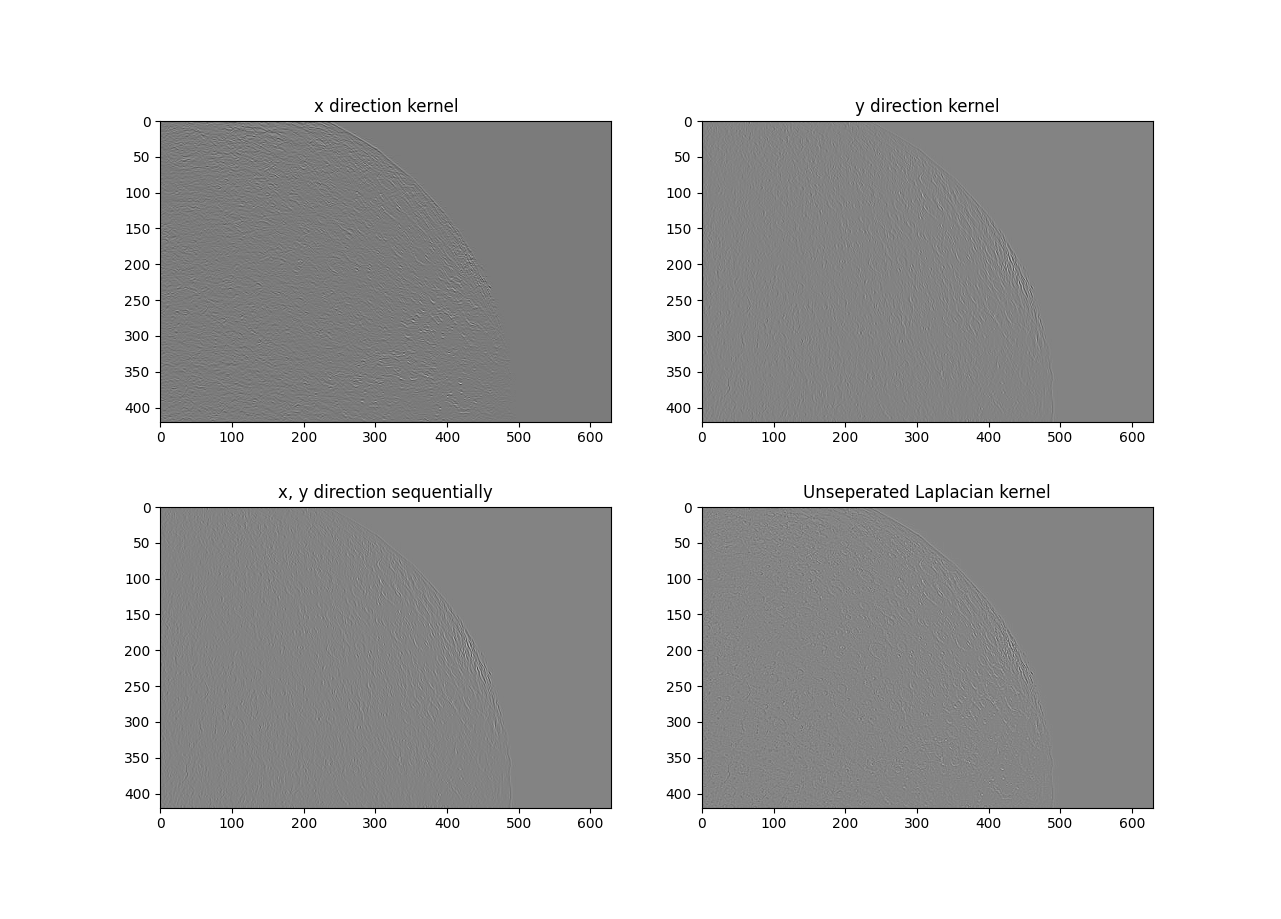
\includegraphics[width=1\textwidth]{../images/p2/p2a.png}
    \caption{Separated Laplacian kernels processed image}
\label{fig:p2a}
\end{figure}


(b) The Sharpened image with Laplacian kernel is shown in Figure \ref{fig:p2b}.\\
\begin{figure}[htbp]
    \centering
    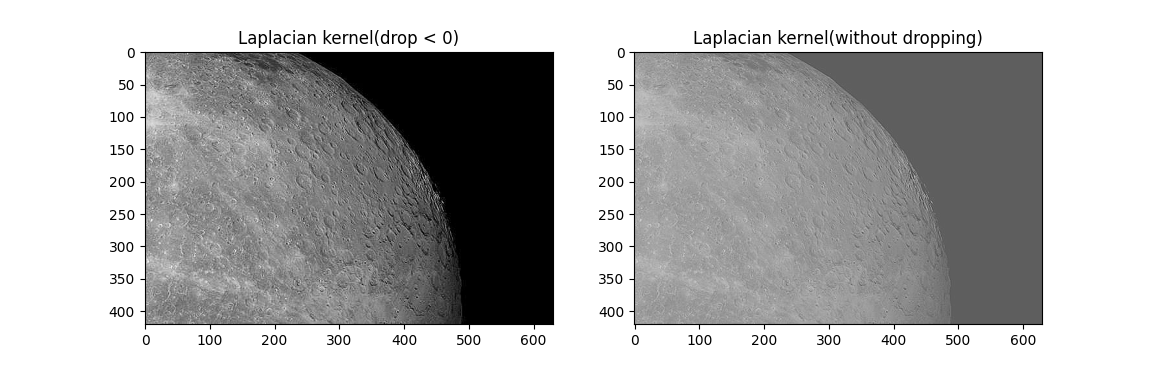
\includegraphics[width=\textwidth]{../images/p2/p2b.png}
    \caption{Unseparated Laplacian kernel processed image}
\label{fig:p2b}
\end{figure}

The image sharpening with Laplacian could be seen as sharpened with the kernel
$$
\begin{bmatrix}
    0 & -1 & 0 \\
    -1 & 5 & -1 \\
    0 & -1 & 0
\end{bmatrix}
$$

In order to make the right side of the image to be black instead of being gray, the $<0$ and $>255$ part are abandoned, i.e. turning the $<0$ part into $0$, and turning the $>255$ part into $255$,
which is shown in the left image.\\
And the right image is doing no additional operations, slighting mapping $[\text{min},\text{max}]\to[0,255]$.\\

(c) The Sharpened image with unsharpen mask is shown in Figure \ref{fig:p2c}.\\
The first two rows (marked filter1 in the title) are smoothed with the kernel 
$$\text{kernel\ 1}=\dfrac{1}{9}\begin{bmatrix}1 & 1 & 1\\1 & 1 & 1\\1 & 1 & 1\end{bmatrix}$$

And the last two rows (marked filter2 in the title) are smoothed with the kernel
$$\text{kernel\ 2}=\dfrac{1}{16}\begin{bmatrix}1 & 2 & 1\\2 & 4 & 2\\1 & 2 & 1\end{bmatrix}$$

Suppose the origin image is $f(x,y)$.\\
The first column are the smoothed images processed by kernel1 and kernel2, mark as $\overline{f(x,y)}$.\\
The second column are the unsharped masks processed by kernel1 and kernel2. i.e. the difference between the
origin image and the smoothed image. i.e. $g_{mask}(x,y)=f(x,y)-\overline{f(x,y)}$.\\
The third and the forth column are the sharpened images with different $k$. i.e. $g(x,y)=f(x,y)+k\cdot g_{mask}(x,y)$\\
The third column is the sharpened image with $k=1$, and the forth column is the sharpened image with $k=4.5$.\\
And the fifth column is the origin image.\\

For the difference bewteen the $1,2$ rows and $3,4$ rows is that: the $1,3$ rows are doing normalization with $[\text{min},\text{max}]\to[0,255]$,
and the $2,4$ rows are setting $<0$ and $>255$ part are abandoned, i.e. turning the $<0$ part into $0$, and turning the $>255$ part into $255$.\\
We could see that as $k$ grows, more high frequency of the image increases, make the image sharper.\\

\begin{figure}[htbp]
    \centering
	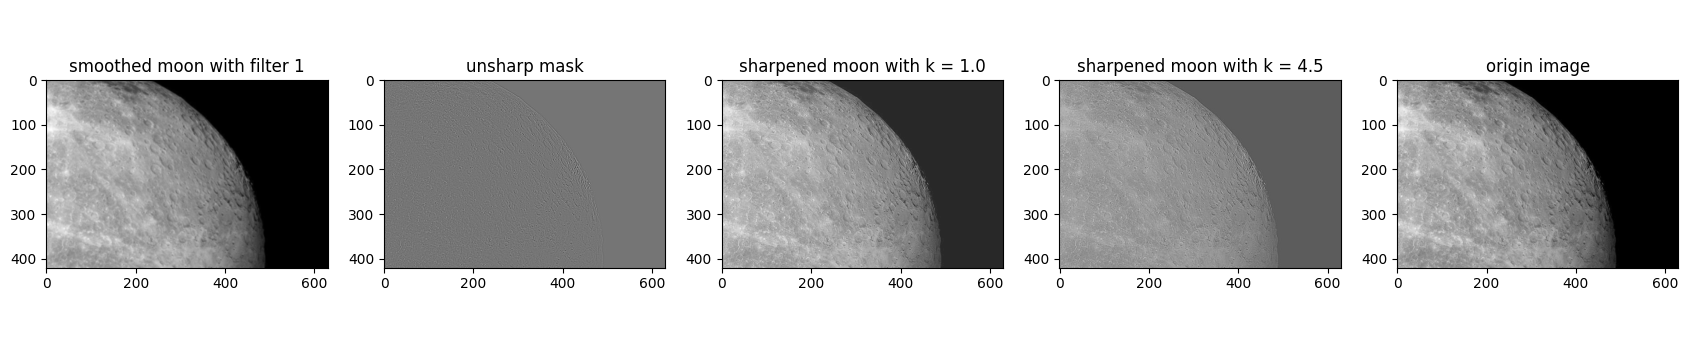
\includegraphics[width=\textwidth]{../images/p2/p2c_1_no_drop.png}
	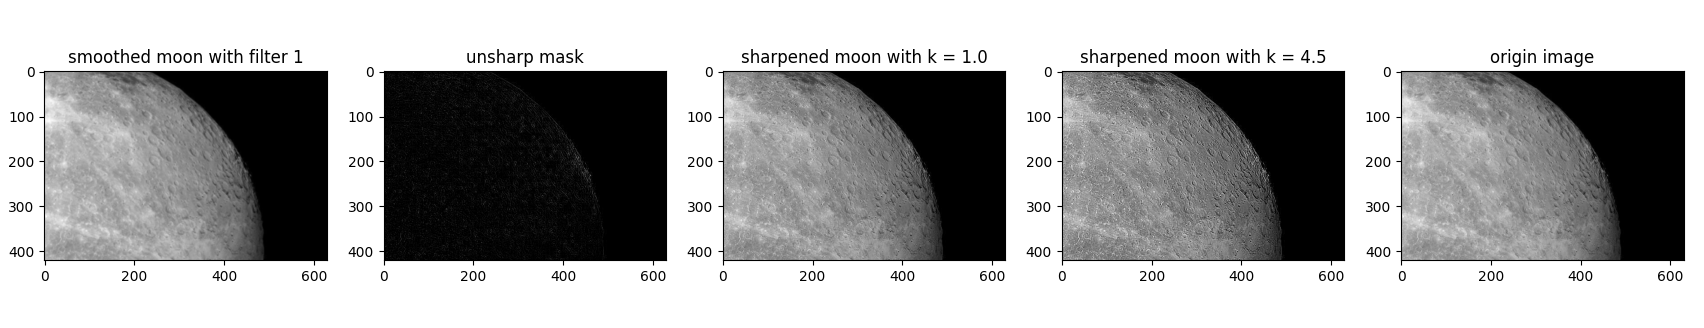
\includegraphics[width=\textwidth]{../images/p2/p2c_1_drop.png}
    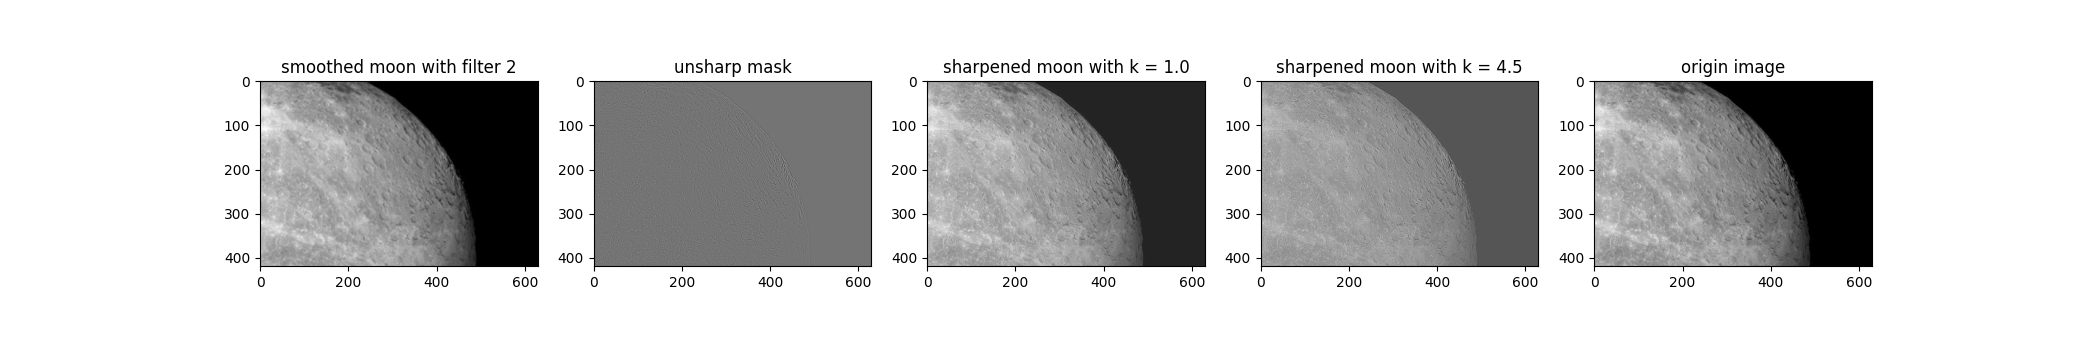
\includegraphics[width=\textwidth]{../images/p2/p2c_2_no_drop.png}
	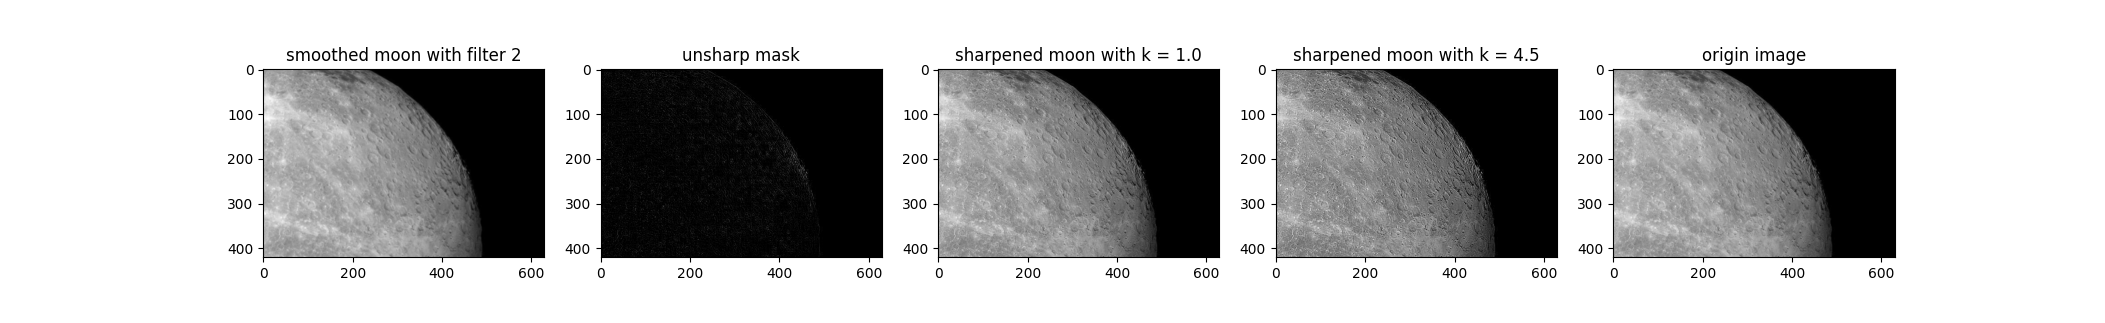
\includegraphics[width=\textwidth]{../images/p2/p2c_2_drop.png}
    \caption{unsharpen mask processed image}
\label{fig:p2c}
\end{figure}

\newpage
\problem{}
The processed image by the median filter is shown in Figure \ref{fig:p3a}.

And we could see that the median kernel with size $3 \times 3$ has the best performance in this case.\\
The kernel has the proper size that remove the salt and pepper noise.

From the result, we could see that all the median filter processed images eliminate the salt and pepper noise, but the kernel size $3 \times 3$ has the best performance. The kernel size $5 \times 5$ and $7 \times 7$ make the 
processed images much blur than the $3 \times 3$ kernel size.

Analyse:


\begin{figure}[htbp]
    \centering
	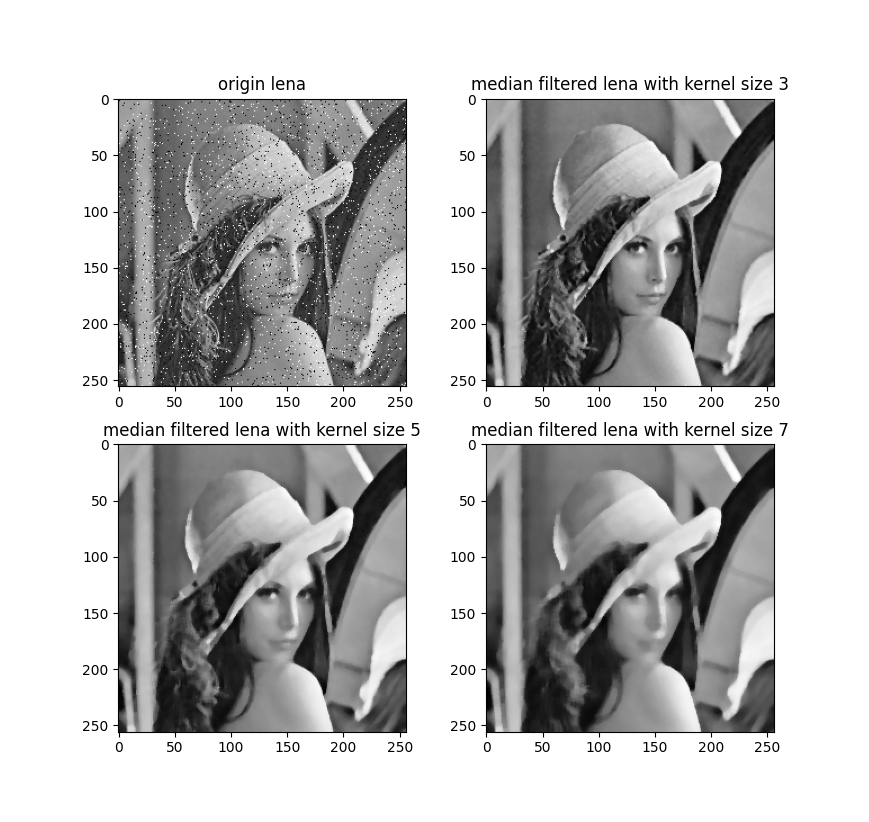
\includegraphics[width=\textwidth]{../images/p3/p3a.png}
    \caption{Median filter processed image}
\label{fig:p3a}
\end{figure}

The processed image by the and Gaussian filter is shown in Figure \ref{fig:p3b}.

Since the Gaussian filter's elements are $G(s,t)=Ke^{-\frac{s^2+t^2}{2\sigma^2}}$, but with the the normalize factor, the value of
$K$ would be eliminate, so $K$ does not matter. So we can just take $K=1$ and adjust the kernel size.

Analyse:


\begin{figure}[htbp]
    \centering
	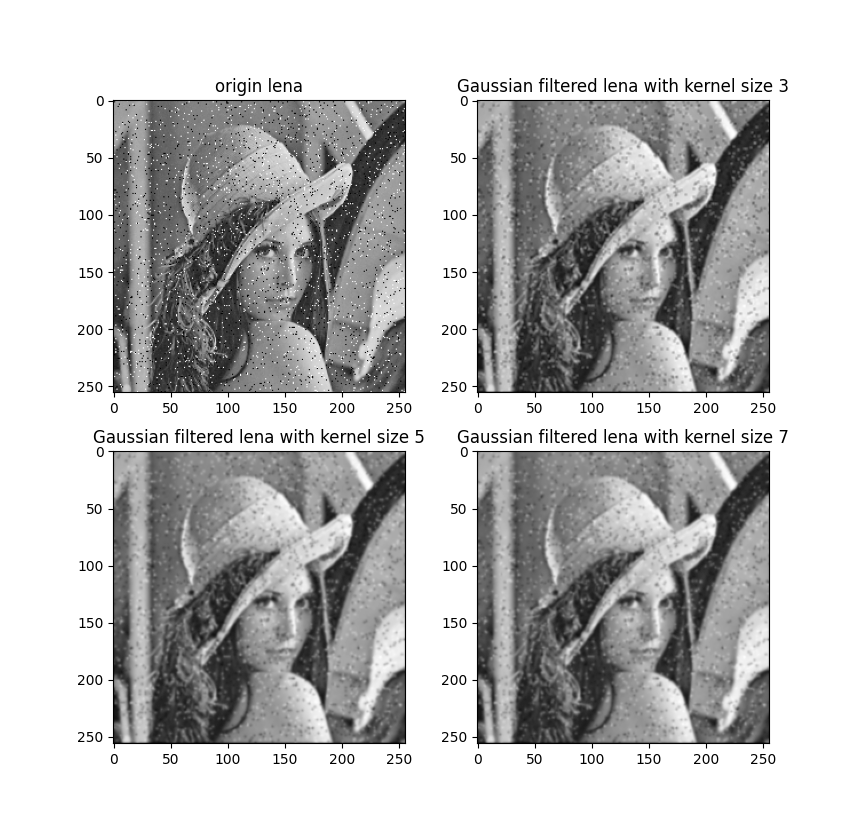
\includegraphics[width=\textwidth]{../images/p3/p3b.png}
    \caption{Gaussian filter processed image}
\label{fig:p3b}
\end{figure}



Salt-and-pepper noise is a common type of image noise characterized by random occurrences of black (pepper) and white (salt) pixels scattered across an image. When dealing with images afflicted by salt-and-pepper noise, median filters and Gaussian filters are two commonly used denoising methods. Each has its characteristics and is suitable for different denoising needs.
Median Filter
Principle: The median filter works by replacing each pixel value with the median value of all pixel values in its neighborhood. This method is particularly effective for removing salt-and-pepper noise since such noise usually consists of extreme values, and the median filter can preserve image edges well.
Different Sizes of Median Filters:
Small-size filters (e.g., 3x3) can effectively remove noise while preserving the sharpness and details of the image. However, for images with a high density of noise, small-size filters may not be sufficient to completely eliminate the noise.
Large-size filters (e.g., 5x5 or larger) are more effective for images with a high noise density because they provide a larger neighborhood for calculating the median. However, using large-size filters may lead to a loss of image detail, making the image appear blurry.
Gaussian Filter
Principle: The Gaussian filter is a linear smoothing filter that replaces each pixel value with a weighted average of its neighboring pixel values, where the weights are determined by a Gaussian function. This gives the greatest weight to the central pixel, with the weight decreasing as the distance from the central pixel increases.
Different Sizes of Gaussian Filters:
Small-size filters (e.g., 3x3) provide a slight smoothing effect that can remove minor noise while maintaining the overall clarity of the image. However, it may not be very effective at removing salt-and-pepper noise, especially at higher noise levels.
Large-size filters (e.g., 5x5 or larger) provide a stronger smoothing effect, more suitable for removing larger areas of noise. However, this comes at the cost of sacrificing image clarity and detail.
Summary
Removing Salt-and-Pepper Noise: Median filters are generally more suited for removing salt-and-pepper noise than Gaussian filters, especially when the noise density is high.
Preserving Edges: Compared to Gaussian filters, median filters are better at preserving image edges while removing noise.
Filter Size Selection: The size of the filter should be chosen based on the density of the noise and the need to preserve image details. Larger filter sizes, although more effective at noise removal, may also lead to a loss of image detail.
In practical applications, the choice of which filter to use and what size to employ often depends on the specific characteristics of the image and denoising requirements, which may need to be determined through experimentation to find the optimal settings.
\problem{Image Restoration}
(a) The spectrum of the origin image is generated through FFT.\\
To shift the zero frequency to the center of the spectrum, we times $(-1)^{u+v}$ for each pixel $(u,v)$ on the origin image before applying FFT.

To have a better effect of visualization on the frequency domain, the image is shown by applying the log transformation on the magnitude of the Fourier transform of the image.\\
i.e. $I_{\text{log}}=20\log(1+|I|)$, where $I$ is the spectrum generated by Fourier transform of the image.

\begin{figure}[htbp]
    \centering
	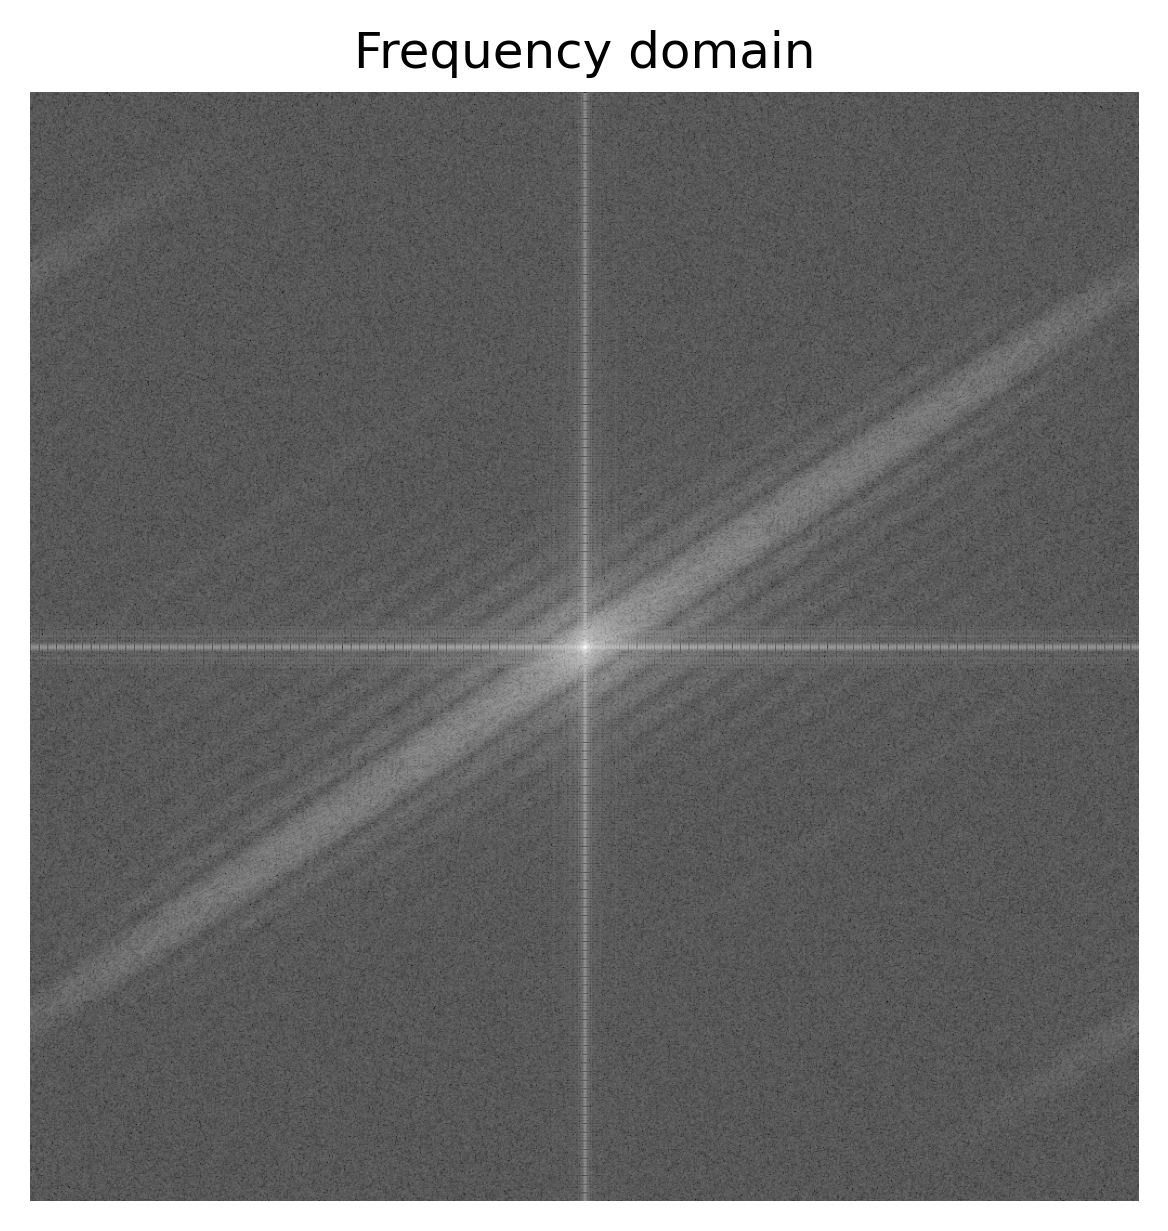
\includegraphics[width=0.5\textwidth]{../images/p4/p4a.png}
    \caption{FFT shifted spectrum}
    \label{fig:p4a}
\end{figure}

(b) The image by applying Radon transform on the origin image is shown in Figure \ref{fig:p4b}.\\
We can get the coordinates with the highest intensity in the Radon transformed image, which is $(\theta,d)=(,)$.\\

So above all, the angle between the strip and the vertical direction is $\theta=$
and the distance between two similar dark strips is $d=$

$N=640,L=\dfrac{N}{d}=$

% \begin{figure}[htbp]
%     \centering
% 	\includegraphics[width=\textwidth]{../images/p4/p4b.png}
%     \caption{Radon Transformed image}
%     \label{fig:p4b}
% \end{figure}




(c)


% \begin{figure}[htbp]
%     \centering
% 	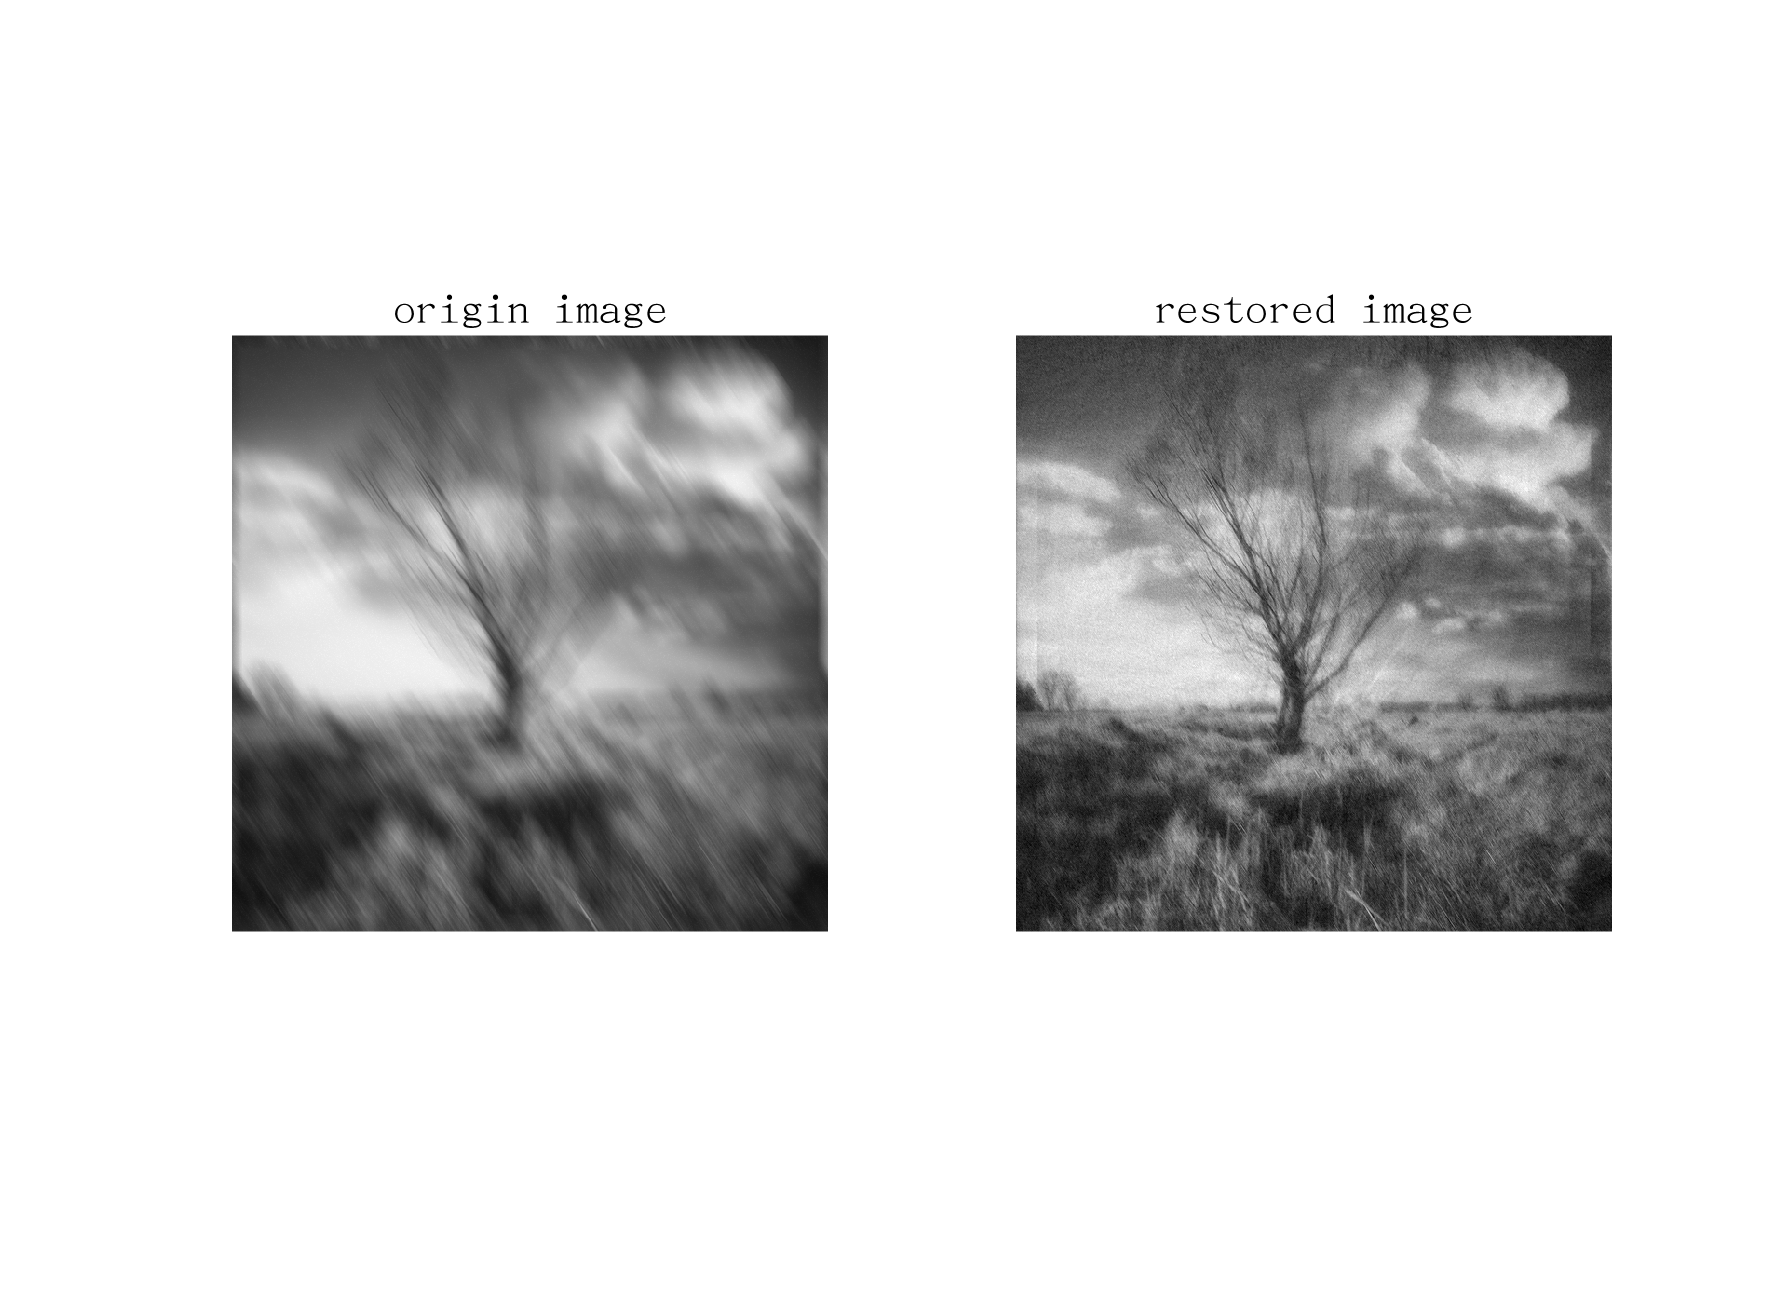
\includegraphics[width=\textwidth]{../images/p4/p4c.png}
%     \caption{p4c}
%     \label{fig:p4c}
% \end{figure}





\newpage

\end{document}